%%%%%%%%%%%%%%%%%%%%%%%%%%%%%%%%%%%%%%%%%
% Beamer Presentation
% LaTeX Template
% Version 1.0 (10/11/12)
%
% This template has been downloaded from:
% http://www.LaTeXTemplates.com
%
% License:
% CC BY-NC-SA 3.0 (http://creativecommons.org/licenses/by-nc-sa/3.0/)
%
%%%%%%%%%%%%%%%%%%%%%%%%%%%%%%%%%%%%%%%%%

%----------------------------------------------------------------------------------------
%	PACKAGES AND THEMES
%----------------------------------------------------------------------------------------

\documentclass{beamer}

\mode<presentation> {

% The Beamer class comes with a number of default slide themes
% which change the colors and layouts of slides. Below this is a list
% of all the themes, uncomment each in turn to see what they look like.

%\usetheme{default}
%\usetheme{AnnArbor}
%\usetheme{Antibes}
%\usetheme{Bergen}
%\usetheme{Berkeley}
%\usetheme{Berlin}
%\usetheme{Boadilla}
%\usetheme{CambridgeUS}
%\usetheme{Copenhagen}
%\usetheme{Darmstadt}
%\usetheme{Dresden}
%\usetheme{Frankfurt}
%\usetheme{Goettingen}
%\usetheme{Hannover}
%\usetheme{Ilmenau}
%\usetheme{JuanLesPins}
%\usetheme{Luebeck}
\usetheme{Madrid}
%\usetheme{Malmoe}
%\usetheme{Marburg}
%\usetheme{Montpellier}
%\usetheme{PaloAlto}
%\usetheme{Pittsburgh}
%\usetheme{Rochester}
%\usetheme{Singapore}
%\usetheme{Szeged}
%\usetheme{Warsaw}

% As well as themes, the Beamer class has a number of color themes
% for any slide theme. Uncomment each of these in turn to see how it
% changes the colors of your current slide theme.

%\usecolortheme{albatross}
%\usecolortheme{beaver}
%\usecolortheme{beetle}
%\usecolortheme{crane}
%\usecolortheme{dolphin}
%\usecolortheme{dove}
%\usecolortheme{fly}
%\usecolortheme{lily}
%\usecolortheme{orchid}
%\usecolortheme{rose}
%\usecolortheme{seagull}
%\usecolortheme{seahorse}
%\usecolortheme{whale}
%\usecolortheme{wolverine}

%\setbeamertemplate{footline} % To remove the footer line in all slides uncomment this line
%\setbeamertemplate{footline}[page number] % To replace the footer line in all slides with a simple slide count uncomment this line

%\setbeamertemplate{navigation symbols}{} % To remove the navigation symbols from the bottom of all slides uncomment this line
}

\usepackage{graphicx} % Allows including images
\usepackage{booktabs} % Allows the use of \toprule, \midrule and \bottomrule in tables
\usepackage{cool}
\usepackage{tikz}
\usepackage{amsmath}
\usepackage{xcolor}
\usepackage{hyperref}
\usepackage{bm}

\DeclareMathOperator*{\argmax}{argmax}
\DeclareMathOperator*{\argmin}{argmin}
\usetikzlibrary{positioning}

%----------------------------------------------------------------------------------------
%	TITLE PAGE
%----------------------------------------------------------------------------------------

\title[RL for Finance]{Reinforcement Learning for Finance} % The short title appears at the bottom of every slide, the full title is only on the title page

\author{Ashwin Rao} % Your name
\institute[Stanford] % Your institution as it will appear on the bottom of every slide, may be shorthand to save space
{Stanford University
 % Your institution for the title page
}

\date{} % Date, can be changed to a custom date

\begin{document}
\begin{frame}
\titlepage % Print the title page as the first slide
\end{frame}

% \begin{frame}
% \frametitle{Overview} % Table of contents slide, comment this block out to remove it
% \tableofcontents % Throughout your presentation, if you choose to use \section{} and \subsection{} commands, these will automatically be printed on this slide as an overview of your presentation
% \end{frame}


\begin{frame}
\frametitle{A bit about me}
\pause
\begin{itemize}[<+->]
\item 1998-2012: Quant at Goldman Sachs and MD at Morgan Stanley
\item 2016-2022: VP of AI at Target (the Retailer)
\item Adjunct Professor, \href{https://icme.stanford.edu/}{\underline{\textcolor{blue}{Applied Math (ICME)}}}, Stanford University
\item I direct Stanford's \href{https://mcf.stanford.edu/}{\underline{\textcolor{blue}{Mathematical \& Computational Finance program}}}
\item Research \& Teaching in: {\em RL and it's applications to Finance \& Retail}
\item Main job: Founder-CTO of an Enterprise AI startup \href{http://cxscore.ai}{\underline{\textcolor{blue}{cxscore.ai}}} 
\end{itemize}
\end{frame}

\begin{frame}
\frametitle{RL For Finance book}
\begin{center}
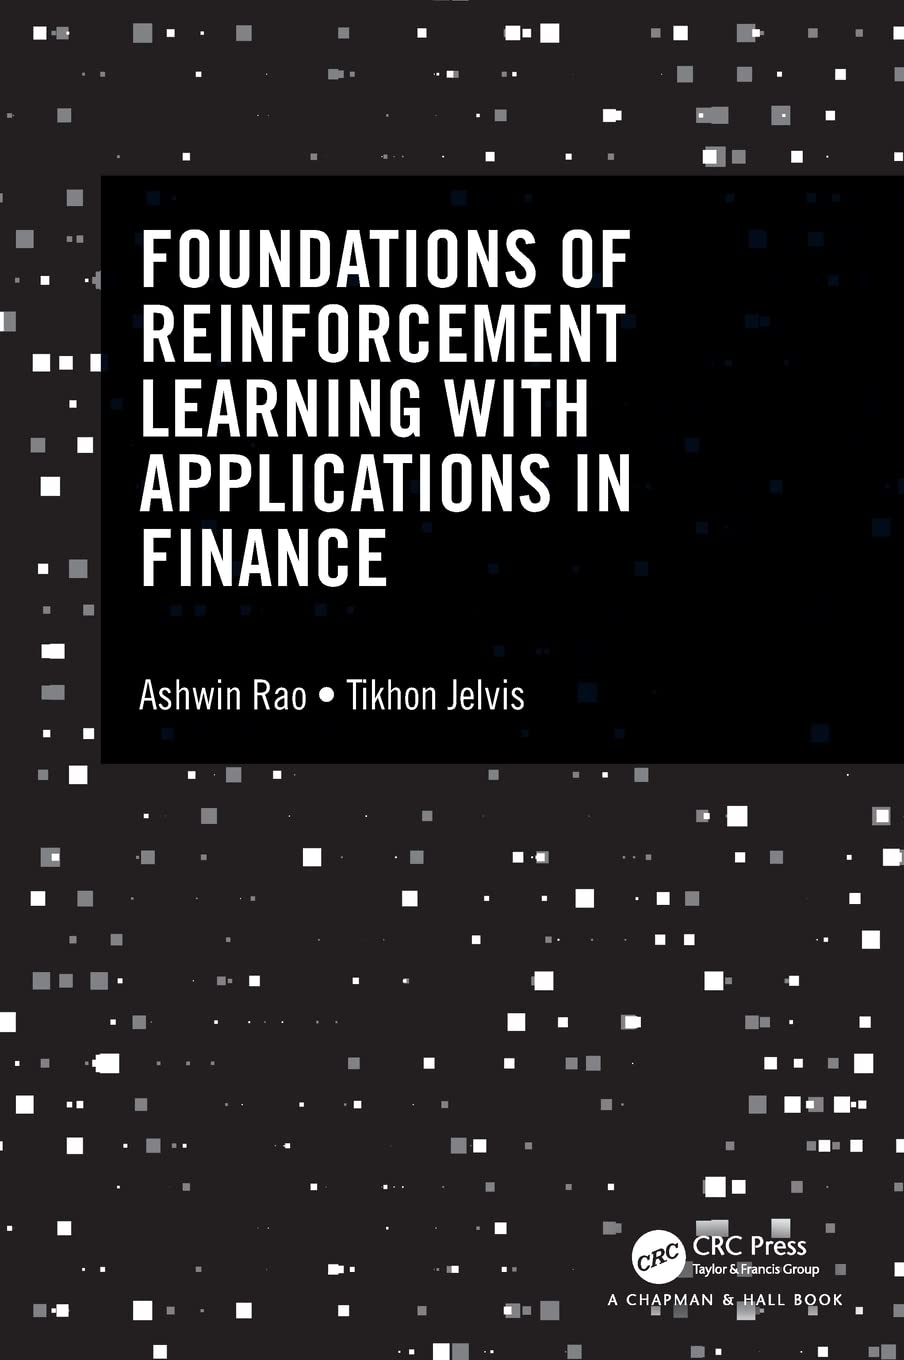
\includegraphics[width=5.5cm, height=8cm]{RLBook.jpeg}
\end{center}
\end{frame}


\begin{frame}
\frametitle{The RL Framework}
\begin{center}
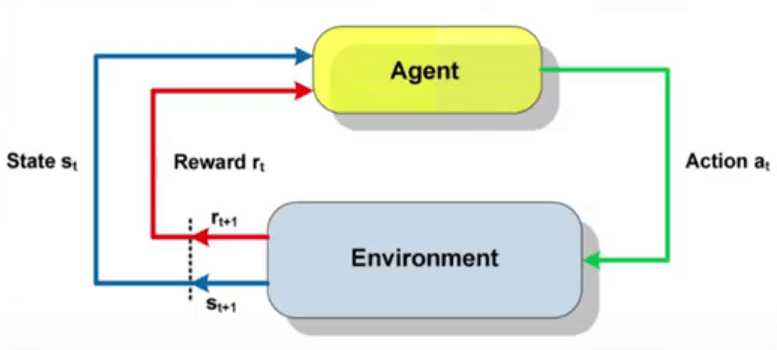
\includegraphics[width=12cm, height=7cm]{RL_diagram.jpg}
\end{center}
\end{frame}

\begin{frame}
\frametitle{Components of the Framework}
\pause
\begin{itemize}[<+->]
\item The {\em Agent} and the {\em Environment} interact in a time-sequenced loop
\item {\em Agent} responds to [{\em State}, {\em Reward}] by taking an {\em Action}
\item {\em Environment} responds by producing next step's (random) {\em State}
\item {\em Environment} also produces a (random) {\em Reward}
\item Goal of {\em Agent} is to maximize {\em Expected Sum} of all future {\em Reward}s
\item This is a dynamic (time-sequenced control) system under uncertainty
\end{itemize}
\end{frame}

\begin{frame}
\frametitle{Many real-world problems fit this framework}
\pause
\begin{itemize}[<+->]
\item Self-driving vehicle (speed/steering to optimize safety/time)
\item Game of Chess (Boolean {\em Reward} at end of game)
\item Complex Logistical Operations (eg: movements in a Warehouse)
\item Make a humanoid robot walk/run on difficult terrains
\item Manage an investment portfolio
\item Control a power station
\item Optimal decisions during a football game
\item Strategy to win an election (highly complex)
\end{itemize}
\end{frame}


\begin{frame}
\frametitle{Dynamic Programming}
\pause
\begin{itemize}[<+->]
\item When Probabilities Model is known $\Rightarrow$ {\em Dynamic Programming} (DP)
\item DP Algorithms take advantage of knowledge of probabilities
\item So, DP Algorithms do not require interaction with the environment
\item In the Language of AI, DP is a type of {\em Planning Algorithm}
\item Why is DP not effective in practice?
\pause
\begin{itemize}[<+->]
\item Curse of Dimensionality
\item Curse of Modeling
\end{itemize}
\item Curse of Dimensionality can be partially cured with Approximate DP
\item To resolve both curses effectively, we need RL
\end{itemize}
\end{frame}

\begin{frame}
\frametitle{Reinforcement Learning}
\pause
\begin{itemize}[<+->]
\item Typically in real-world, we don't have access to a Probabilities Model
\item All we have is access to an environment serving individual experiences
\item RL interacts with either {\em actual} or {\em simulated} environment
\item RL is a ``trial-and-error'' approach linking {\em Actions} to {\em Returns}
\item Try different actions \& learn what works, what doesn't
\item RL incrementally learns from a stream of data through interactions
\item Big Picture: Sampling and Function Approximation come together
\item Deep Neural Networks are typically used for function approximation
\end{itemize}
\end{frame}

\begin{frame}
\frametitle{Reinforcement Learning}
\pause
\begin{itemize}[<+->]

\item {\bf Promise of modern A.I. is based on success of RL algorithms}
\item Potential for automated decision-making in many industries
\item In ~10 years: Bots that act or behave more optimal than humans
\item RL already solves various low-complexity real-world problems
\item Journey from GPT to ChatGPT was enabled by RL
\item Possibilities in Finance are endless (I will cover 2 problems)
\end{itemize}
\end{frame}


\begin{frame}
\frametitle{P1: Dynamic Asset-Allocation and Consumption}
\pause
\begin{itemize}[<+->]
\item The broad topic is Investment Management
\item Applies to Corporations as well as Individuals
\item The two considerations are:
\pause
\begin{itemize}[<+->]
\item How to allocate money across assets in one's investment portfolio
\item How much to consume for one's needs/operations/pleasures
\end{itemize}
\item We consider the dynamic version of these dual considerations
\item Asset-Allocation and Consumption decisions at each time step
\item Asset-Allocation decisions typically deal with Risk-Reward tradeoffs
\item Consumption decisions are about spending now or later
\item Objective: Horizon-Aggregated Expected \href{https://github.com/coverdrive/technical-documents/blob/master/finance/cme241/Tour-UtilityTheory.pdf}{\underline{\textcolor{blue}{Utility of Consumption}}}
\end{itemize}
\end{frame}

\begin{frame}
\frametitle{Consider the simple example of Personal Finance}
\pause
\begin{itemize}[<+->]
\item Broadly speaking, Personal Finance involves the following aspects:
\pause
\begin{itemize}[<+->]
\item Receiving Money: Salary, Bonus, Rental income, Asset Liquidation etc.
\item Consuming Money: Food, Clothes, Rent/Mortgage, Car, Vacations etc.
\item Investing Money: Savings account, Stocks, Real-estate, Gold etc.
\end{itemize}
\item Goal: Maximize lifetime-aggregated Expected Utility of Consumption
\item We can model this in the RL framework as follows:
\item {\em State:} Age, Asset Holdings, Asset Valuation, Career situation etc.
\item {\em Action:} Changes in Asset Holdings, Optional Consumption
\item {\em Reward:} Utility of Consumption of Money
\item {\em Model:} Career uncertainties, Asset market uncertainties
\end{itemize}
\end{frame}


\begin{frame}
\frametitle{Trading Order Book (abbrev. OB)}
\includegraphics[width=11.5cm, height=7cm]{cme241/order_book.png}
\end{frame}

\begin{frame}
\frametitle{Order Book Dynamics and Price Impact}
\pause
\begin{itemize}[<+->]
\item Buyers/Sellers express their intent to trade by submitting bids/asks
\item These are Limit Orders (LO) with a price $P$ and size $N$
\item Buy LO $(P, N)$ states willingness to buy $N$ shares at a price $\leq P$
\item Sell  LO $(P, N)$ states willingness to sell $N$ shares at a price $\geq P$
\item A Market Order (MO) states intent to buy/sell $N$ shares at the {\em best possible price(s)} available on the OB at the time of MO submission
\item A Sell Market Order will remove the best bid prices on the OB
\item A large-sized MO can result in a big {\em Big-Ask Spread} - we call this the {\em Temporary Price Impact}
\item {\em Spread} typically replenished by new LOs, potentially from either side
\item Subsequent Replenishment moves {\em Bid/Ask Stacks} - we call this the {\em Permanent Price Impact}
\item Price Impact Models with OB Dynamics can be quite complex
\end{itemize}
\end{frame}


\begin{frame}
\frametitle{Stylized Example of an Order Book}
\includegraphics[width=13cm, height=8cm]{order_book_0.png}
\end{frame}

\begin{frame}
\frametitle{Sell Limit Order: 40 Shares @ 107 Price}
\includegraphics[width=13cm, height=8cm]{order_book_1.png}
\end{frame}

\begin{frame}
\frametitle{Sell Market Order: 120 Shares}
\includegraphics[width=13cm, height=8cm]{order_book_2.png}
\end{frame}

\begin{frame}
\frametitle{Buy Limit Order: 80 shares @ 100 Price}
\includegraphics[width=13cm, height=8cm]{order_book_3.png}
\end{frame}

\begin{frame}
\frametitle{Sell Limit Order: 60 shares @ 104 Price}
\includegraphics[width=13cm, height=8cm]{order_book_4.png}
\end{frame}

\begin{frame}
\frametitle{Buy Market Order: 150 shares}
\includegraphics[width=13cm, height=8cm]{order_book_5.png}
\end{frame}

\begin{frame}
\frametitle{Optimal Trade Order Execution Problem}
\pause
\begin{itemize}[<+->]
\item The task is to sell a large block of shares in a finite amount of time
\item We are only allowed to submit Market Orders
\item Need to consider both {\em Temporary} and {\em Permanent} Price Impact
\item Goal is to maximize Risk-Adjusted Total Sales Proceeds
\item By breaking the block into appropriate chunks (timed appropriately)
\item If we sell too fast, we are likely to get poor prices
\item If we sell too slow, we risk running out of time
\item Selling slowly leads to more uncertain proceeds (``risk-adjustment'')
\item This is a Dynamic Optimization problem
\end{itemize}
\end{frame}

\begin{frame}
\frametitle{Modeling in the RL framework}
\pause
\begin{itemize}[<+->]
\item {\em State} is current bid/ask stacks, and shares not yet sold
\item {\em Action} is number of shares to be sold at this instant
\item {\em Reward} is Utility of {\bf price-impacted} sale proceeds
\item Utility function does ``risk-adjustment'' of uncertain proceeds
\item {\em Model} comprises of {\em Temporary} and {\em Permanent} Price Impact
\item An RL algorithm will learn and optimize using a {\em simulated} OB
\item The {\em simulated} OB is learnt by observing real OB dynamics
\end{itemize}
\end{frame}

\begin{frame}
\frametitle{Other Problems in my Book}
\pause
\begin{itemize}[<+->]
\item Optimal Market-Making in an Order Book
\begin{itemize}
\item Dynamic adjustment of bid and ask prices/sizes
\item Anticipating Price Impact 
\end{itemize}
\item Derivatives Pricing and Hedging in an Incomplete Market
\begin{itemize}
\item Playing the game of Dynamic Portfolio Optimization with Hedges
\end{itemize}
\item Optimal Exercise of American Options
\begin{itemize}
\item Treated as an Optimal Stopping Problem (modeled as MDP)
\item Computational Efficiency for High-Dimensional American Options
\end{itemize}
\end{itemize}
\end{frame}

\end{document}